\documentclass[11pt,letterpaper]{article}
\usepackage[T1]{fontenc}
\usepackage[utf8]{inputenc}
\usepackage[spanish,es-nodecimaldot]{babel}
\usepackage{lmodern,graphicx,tabularx,booktabs,array,caption,fancyhdr,titlesec}
\usepackage[table]{xcolor}
\usepackage[letterpaper,left=24mm,right=24mm,top=24mm,bottom=22mm,headheight=15pt]{geometry}
\usepackage[hidelinks]{hyperref}
\definecolor{vino}{HTML}{7A1F2B}\definecolor{titulo}{HTML}{551620}\definecolor{rosa}{HTML}{F5EDEE}
\renewcommand{\familydefault}{\sfdefault}
\titleformat{\section}{\Large\bfseries\color{titulo}}{\thesection.}{.4em}{}
\titleformat{\subsection}{\large\bfseries\color{vino}}{\thesubsection.}{.4em}{}
\titlespacing*{\subsection}{0pt}{11pt}{3pt}
\setlength{\parindent}{0pt}\setlength{\parskip}{5pt}
\pagestyle{fancy}\fancyhf{}\fancyhead[R]{\small\color{vino}UNSAAC · Ingeniería Informática y de Sistemas}
\fancyfoot[L]{\small Desarrollo de Software II · IF616BIN}\fancyfoot[R]{\small Sesión 3 · Página \thepage}
\renewcommand{\headrulewidth}{.4pt}
\renewcommand{\arraystretch}{1.28}
\newcommand{\tabla}[2]{\par\smallskip\begin{tabularx}{\linewidth}{@{}>{\bfseries\color{vino}}p{.28\linewidth}X@{}}\toprule\rowcolor{rosa}#1\\\midrule #2\bottomrule\end{tabularx}\par}
\newcommand{\ruta}[1]{\nolinkurl{#1}}
\newcommand{\foto}[3]{\begin{minipage}[t]{.48\linewidth}\centering\includegraphics[height=#1,keepaspectratio]{evidencias/#2}\captionof{figure}{#3}\end{minipage}}
\captionsetup{font=small,labelfont=bf,hypcap=false}
\begin{document}
\begin{titlepage}\centering
{\color{vino}\bfseries UNIVERSIDAD NACIONAL DE SAN ANTONIO ABAD DEL CUSCO\\[4pt]
\small FACULTAD DE INGENIERÍA ELÉCTRICA, ELECTRÓNICA, INFORMÁTICA Y MECÁNICA\\
ESCUELA PROFESIONAL DE INGENIERÍA INFORMÁTICA Y DE SISTEMAS\par}
\vspace{5mm}

\includegraphics[height=2cm]{evidencias/insignia.png}\hspace{1cm}
\includegraphics[height=2cm]{evidencias/escuela.jpg}\par
\vfill
{\LARGE\bfseries\color{titulo} DESARROLLO DE SOFTWARE II\par}
Código IF616BIN — Semestre Académico 2026-II\par
\vspace{6mm}
{\large\bfseries\color{titulo} INFORME DE PRÁCTICA — SESIÓN 3\par}
{\Large\bfseries\color{titulo} Autenticación con Firebase y sesión con BLoC\\Wallet UNSAAC\par}
\vspace{4mm}
Segunda Unidad Didáctica · Integración con servicios web y APIs\\
Sesión 3 · lunes 16 de noviembre de 2026\par
\vfill
\raggedright
\tabla{Asignatura & Desarrollo de Software II}{Código & IF616BIN\\Unidad / sesión & Unidad II — Sesión 3\\Producto & Registro, acceso, perfil y recuperación de sesión\\Evaluación & Avance de D2 · tres retos formativos · cierre en la sesión 4\\Modalidad & Individual\\Docente & Mtro. Ing. Yover Collantes Valer\\Estudiante & Axel Barnaby Aranibar Rojas · 220547\\}
\vfill\centering Escuela Profesional de Ingeniería Informática y de Sistemas\\Semestre Académico 2026-II · Cusco, Perú
\end{titlepage}
\section{Datos generales}
\tabla{Campo & Información}{Estudiante & Axel Barnaby Aranibar Rojas · 220547\\Escuela profesional & Ingeniería Informática y de Sistemas\\Asignatura & Desarrollo de Software II (IF616BIN)\\Unidad y sesión & Unidad II · Sesión 3 · 16 de noviembre de 2026\\Docente & Mtro. Ing. Yover Collantes Valer\\Repositorio & \url{https://github.com/axelIn06/wallet-unsaac-aranibar-rojas/tree/sesion-03}\\Revisión de la aplicación & \texttt{1693fd0} · base de la sesión 2: \texttt{7752d93}\\Fecha del informe & 24 de noviembre de 2026\\Alcance & Taller de autenticación y tres retos de ampliación\\}
\section{Resumen del trabajo}
En esta práctica se incorporó autenticación por correo y contraseña a Wallet UNSAAC. Una persona puede crear una cuenta, iniciar sesión y acceder a la billetera. Al cerrar la sesión, la pantalla vuelve al formulario de acceso. La aplicación recibe los cambios de identidad mediante un flujo de Firebase y conserva el formulario durante las operaciones pendientes. La validación del correo, la longitud de la contraseña y la confirmación del registro se ejecutan antes de enviar la solicitud.

Los tres retos amplían ese recorrido. La recuperación presenta el mismo mensaje para direcciones registradas y desconocidas. La edición del perfil cambia el nombre visible y su inicial mientras conserva el identificador del usuario. La pérdida de una sesión devuelve al acceso con un aviso distinto del cierre voluntario. La verificación combinó pruebas unitarias y de widgets con un recorrido en Android conectado al emulador oficial de Authentication. Se comprobó la persistencia cerrando por completo el proceso y abriendo nuevamente la aplicación. La simulación en memoria permite repetir las pruebas sin red.

\textbf{Palabras clave.} Firebase Authentication, BLoC, identidad, sesión, pruebas.
\newpage
\section{Entorno y verificaciones}
\subsection{Versiones utilizadas}
\tabla{Herramienta & Entorno de la práctica}{Flutter y Dart & Flutter 3.41.6 y Dart 3.11.4 en macOS.\\Android & AVD Medium Phone, API 36.1, arm64. Paquete \ruta{pe.edu.unsaac.wallet_unsaac}.\\Firebase & \ruta{firebase_auth} 7.0.1, \ruta{firebase_core} 5.1.0 y Authentication Emulator en el puerto 9099.\\BLoC y compilación & \ruta{flutter_bloc} 9.1.1, Kotlin 2.3.0 y destino JVM 17.\\}
\subsection{Comandos ejecutados}
\tabla{Verificación & Resultado}{Dependencias & Flutter resolvió las versiones de Firebase de la guía y actualizó \ruta{pubspec.lock}.\\Análisis y pruebas & \ruta{flutter analyze --no-pub} sin observaciones. \ruta{flutter test --no-pub} completó 71 pruebas.\\Ejecución & \ruta{flutter run} con \ruta{AUTH_EMULATOR=true} compiló e instaló el APK en el AVD.\\}
\begin{center}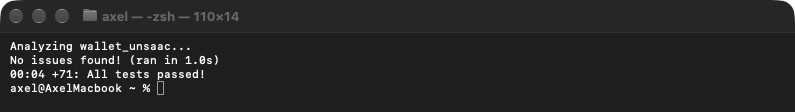
\includegraphics[width=.88\linewidth]{evidencias/consola.png}
\captionof{figure}{Resultado del análisis y contador final de la suite en Terminal.}\end{center}
\subsection{Estructura del repositorio}
\ruta{lib/features/auth/domain/} define el usuario y el contrato de autenticación. \ruta{data/} contiene los dos repositorios. \ruta{presentation/} coordina eventos, estados, formularios y menú de cuenta. Las nuevas pruebas están en \ruta{test/auth/}, y las salidas completas en \ruta{evidencias/sesion-03/}.
\newpage
\subsection{Taller guiado: del formulario a la billetera}
El formulario comprueba el formato del correo y exige seis caracteres como mínimo. Para registrarse también se debe repetir la contraseña. El botón de envío muestra un indicador y se deshabilita mientras el bloc espera. Un error conserva los campos para que el usuario pueda corregirlos.
\begin{center}
\foto{10.2cm}{acceso.png}{Entrada a Wallet UNSAAC con acceso al registro y a la recuperación.}\hfill
\foto{10.2cm}{registro.png}{Registro de una cuenta ficticia en Android. Ambos campos de contraseña están ocultos.}
\end{center}
\textbf{Recorrido de datos.} El formulario envía el evento de registro. El repositorio invoca al SDK y convierte su respuesta en una entidad \texttt{AuthUser}. Al recibir una identidad, \texttt{AuthGate} monta la billetera correspondiente al UID.

\textbf{Decisión de seguridad.} El estado de presentación contiene UID, correo y nombre. Las credenciales se utilizan para la operación de acceso o registro. El SDK administra la sesión y su persistencia. Los movimientos de la práctica siguen en memoria y se crea una billetera nueva al cambiar de usuario.
\newpage
\section{Reto 1 — Recuperación de contraseña}
\subsection{Objetivo y alcance}
Solicitar instrucciones de recuperación desde el acceso y dar una respuesta comprensible sin revelar si una cuenta está registrada.
\subsection{Diseño de la solución}
\tabla{Elemento & Decisión y justificación}{Contrato & \texttt{sendPasswordResetEmail} acepta el correo y finaliza sin devolver información sobre el usuario.\\Presentación & El enlace «¿Olvidaste tu contraseña?» cambia al formulario de recuperación. Solo se valida el correo.\\Fallo operativo & Un problema de red muestra una indicación para reintentar. La ausencia de una cuenta mantiene la confirmación genérica.\\}
\subsection{Implementación}
\texttt{AuthPasswordResetRequested} pasa el correo al repositorio. El adaptador Firebase utiliza la operación del mismo nombre del SDK. El repositorio en memoria simula la respuesta. El texto de confirmación es común a ambas implementaciones.
\begin{verbatim}
await auth.sendPasswordResetEmail(email: email.trim());
\end{verbatim}
\subsection{Pruebas ejecutadas}
\tabla{Caso & Comprobación}{Correo existente y ausente & Dos pruebas del bloc esperan el mismo estado y el mismo mensaje.\\Error de red & El repositorio de prueba lanza un fallo de conexión. El estado comunica el problema.\\Interfaz & Se abre el enlace, se escribe un correo y se comprueba la confirmación en pantalla.\\}
\newpage
\subsection{Evidencias}
\begin{center}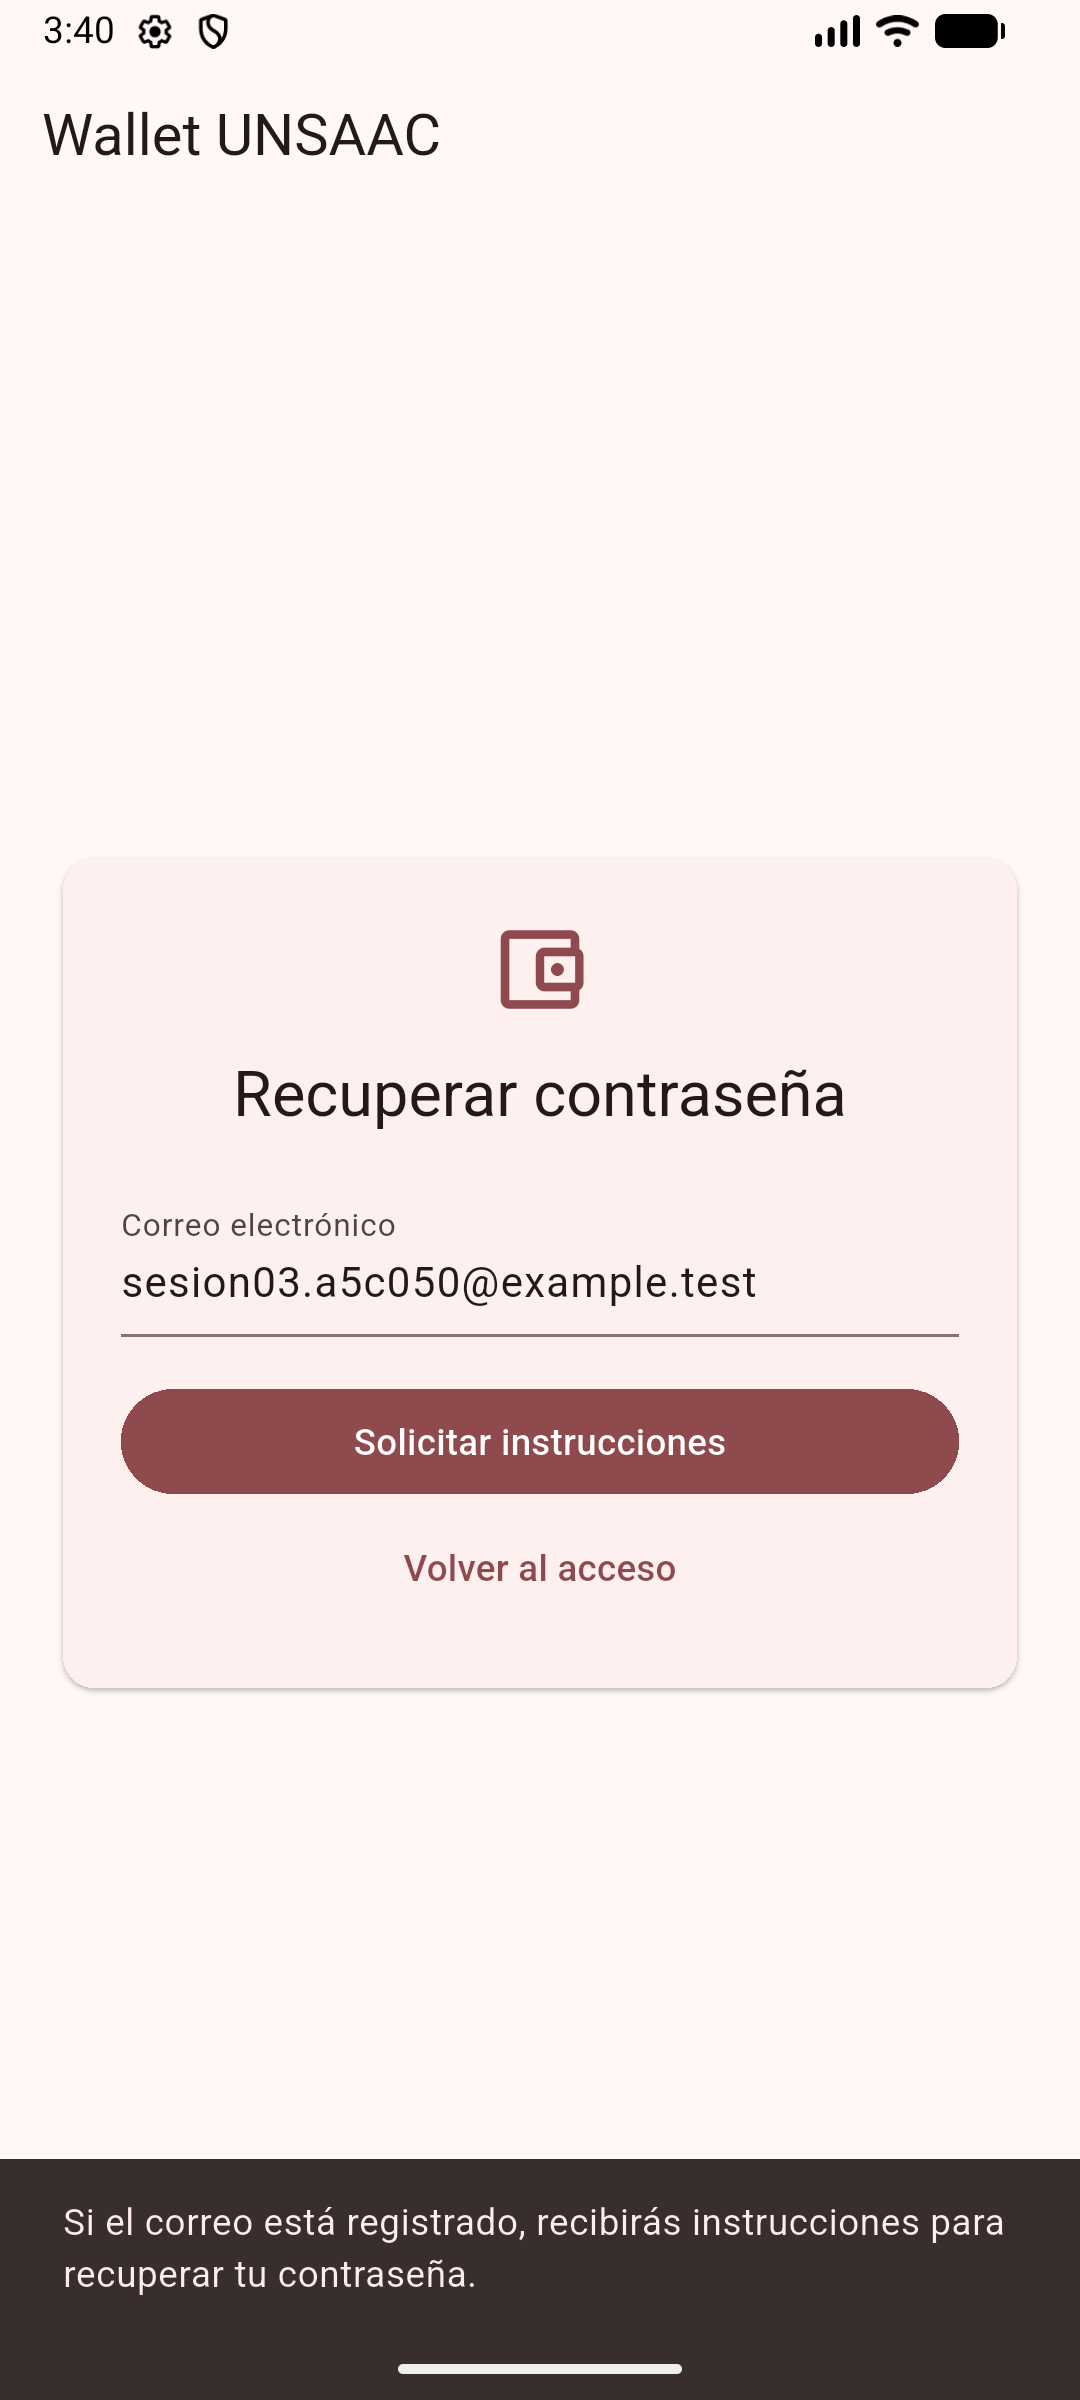
\includegraphics[height=10.2cm]{evidencias/recuperacion.png}
\captionof{figure}{Confirmación de recuperación en Android después de solicitar instrucciones para la cuenta de prueba.}\end{center}
\begin{center}
\includegraphics[width=.72\linewidth]{evidencias/recuperacion-detalle.png}\end{center}
\subsection{Dificultades y decisiones}
La confirmación visual por sí sola podría provenir de una simulación. Se consultó también el servidor local de Authentication y se comprobó que había generado una solicitud de tipo \texttt{PASSWORD\_RESET} para el correo utilizado. El registro de verificación conserva el resultado sin incluir el código ni el enlace de recuperación. El emulador permite comprobar la solicitud sin entregar correo a un buzón.
\subsection{Autoevaluación}
\tabla{Criterio & Evidencia}{Privacidad del correo & Mismo texto para cuenta presente y ausente en las pruebas del bloc.\\Solicitud al proveedor & Tipo de operación comprobado en el emulador oficial.\\Tratamiento de errores & Prueba de fallo del repositorio y mensaje legible.\\}
\newpage
\section{Reto 2 — Perfil con nombre para mostrar}
\subsection{Objetivo y alcance}
Permitir que el usuario cambie su nombre visible sin perder su identidad ni tener que iniciar sesión nuevamente.
\subsection{Diseño de la solución}
\tabla{Elemento & Decisión y justificación}{Identidad & El UID permanece estable. La igualdad por valor incluye UID, correo y nombre.\\Edición & El menú de cuenta abre un formulario con el nombre actual. La entrada se recorta; un nombre vacío se rechaza.\\Presentación & La barra muestra el nombre y su inicial. Si aún no se definió un nombre, utiliza el correo.\\}
\subsection{Implementación}
El formulario envía \texttt{AuthNameRequested}. El adaptador llama a \texttt{updateDisplayName}, conserva el UID y construye una entidad nueva. El bloc comprueba que sigue activa la misma cuenta antes de emitir el resultado. En el modo de práctica se actualiza la cuenta correspondiente dentro del repositorio en memoria.
\begin{verbatim}
await user.updateDisplayName(name.trim());
return AuthUser(user.uid, user.email ?? '', name.trim());
\end{verbatim}
\subsection{Pruebas ejecutadas}
\tabla{Caso & Resultado}{Nombre con espacios & La prueba compara las entidades de antes y después. El nombre queda recortado y ambos UID coinciden.\\Nombre vacío & El bloc conserva el usuario y emite un mensaje que pide escribir un nombre.\\Consulta al proveedor & El servidor de pruebas devuelve el mismo UID de la cuenta creada y el nombre «Axel».\\}
\newpage
\subsection{Evidencias}
\noindent\foto{10.2cm}{perfil.png}{Perfil actualizado. El encabezado muestra «Axel» y el avatar muestra su inicial.}\hfill
\foto{10.2cm}{restaurada.png}{Una segunda captura, tras detener y abrir el proceso Android, muestra el mismo perfil.}
\subsection{Dificultades y decisiones}
Cambiar un texto de la pantalla no demostraría que el cambio llegó a la cuenta. Se comparó el UID del registro con el que devolvió Authentication después de editar el perfil. Luego se detuvo el proceso con \ruta{adb shell am force-stop} y se abrió nuevamente la actividad. El servidor de Authentication permaneció activo durante el reinicio.
\subsection{Autoevaluación}
\tabla{Criterio & Evidencia}{Identidad estable & Comparación del UID en el bloc y consulta al emulador.\\Nombre e inicial & Captura del encabezado tras guardar.\\Restauración de sesión & La billetera reaparece con el perfil actualizado sin introducir credenciales.\\}
\newpage
\section{Reto 3 — Mensajes de sesión y expiración}
\subsection{Objetivo y alcance}
Distinguir la salida que solicita el usuario de la pérdida de una sesión previamente válida. Ante un fallo de cierre o una desconexión temporal, se mantiene la identidad que el SDK todavía reconoce.
\subsection{Diseño de la solución}
\tabla{Situación & Respuesta}{Inicio sin sesión & El primer valor nulo del flujo muestra el formulario de acceso.\\Cierre voluntario & El usuario confirma «Salir». Al cerrarse la sesión se informa «Cerraste sesión».\\Pérdida externa & Si una identidad activa pasa a nula sin petición de salida, se muestra «Tu sesión expiró» y la acción «Volver a iniciar sesión».\\Fallo de red & La comprobación al volver a primer plano conserva la cuenta y muestra el error.\\}
\subsection{Implementación}
\texttt{AuthStarted} se suscribe a \texttt{authStateChanges()}. El bloc recuerda la última identidad observada y si existe una petición explícita de cierre. Al reanudar Android se vuelve a consultar el usuario mediante \texttt{reload()}. Si el proveedor confirma que la cuenta quedó deshabilitada o que la sesión es inválida, el repositorio cierra la sesión.
\subsection{Pruebas ejecutadas}
\tabla{Caso & Resultado}{Expiración por el flujo & El doble de prueba emite una pérdida externa de usuario. El bloc la identifica como expiración y el widget retira la billetera.\\Cierre fallido & El estado conserva el usuario y muestra el mensaje.\\Reanudación & Dos pruebas distinguen una identidad inválida de un fallo de red. Solo la primera vuelve al acceso.\\}
\newpage
\begingroup\small\renewcommand{\arraystretch}{1.08}\subsection{Evidencias}
\noindent\foto{8.6cm}{cierre.png}{Cierre voluntario. El usuario debe confirmar la salida desde el menú de cuenta.}\hfill
\foto{8.6cm}{expiracion.png}{Tras deshabilitar la cuenta ficticia en el servidor de pruebas y reanudar Android, aparece «Tu sesión expiró» con la acción de retorno.}
\begin{center}
\includegraphics[width=.62\linewidth]{evidencias/expiracion-detalle.png}\end{center}
\subsection{Dificultades y decisiones}
Tanto el primer arranque como una expiración pueden producir un usuario nulo. Para diferenciarlos se considera si antes existía una identidad activa. El fallo de una solicitud de red tampoco basta para invalidar al usuario. Las pruebas controlan estos casos de manera independiente.
\subsection{Autoevaluación}
\tabla{Criterio & Evidencia}{Salida y expiración distinguibles & Pruebas del bloc con mensajes diferentes.\\Recuperación desde la interfaz & La prueba de widget ejecuta «Volver a iniciar sesión» y localiza el formulario.\\Gestión de tokens & El almacenamiento de sesión corresponde al SDK. La aplicación no guarda tokens ni contraseñas en preferencias.\\}
\endgroup\newpage
\section{Verificación del avance de D2}
\tabla{Punto de la guía & Evidencia de aceptación}{Registro, acceso y cierre & Recorrido del APK Android contra Firebase Authentication Emulator.\\Persistencia & Detención completa del proceso, nueva apertura y comprobación de identidad.\\Decisión de pantalla & \texttt{AuthGate} representa espera inicial, acceso o billetera.\\Errores comprensibles & Trece casos de validación y traducción. Incluyen código desconocido y credenciales inválidas.\\BLoC y widgets & Diecisiete pruebas del bloc y cinco de interfaz de autenticación. Se conservan las 36 pruebas anteriores.\\README y configuración & Comandos independientes para memoria, SDK con emulador y proyecto personal.\\}
\textbf{Alcance de Firebase.} El proyecto de pruebas es \ruta{demo-wallet-unsaac}. El uso del SDK, la persistencia y las solicitudes al proveedor se verificaron en el emulador. La habilitación de Email/Password en la consola de un proyecto personal queda pendiente de acceso del titular.
\section{Conclusiones y aprendizajes}
\begin{enumerate}
\item El primer evento de identidad permite reconstruir la billetera tras un reinicio. La prueba en Android recuperó el perfil «Axel» sin pedir de nuevo la contraseña.
\item La separación entre el contrato de autenticación y sus adaptadores permitió probar respuestas de red y pérdidas de sesión de forma determinista. El mismo formulario funcionó contra el proveedor emulado.
\item La recuperación necesita dos verificaciones complementarias. La interfaz protege la existencia de la cuenta y el servidor de pruebas acredita que se creó la solicitud.
\end{enumerate}
\newpage
\section{Declaración de originalidad y uso de herramientas de IA}
Se utilizó OpenAI Codex para adaptar el proyecto anterior, implementar los flujos, redactar pruebas, operar el emulador y elaborar el informe en LaTeX. Las capturas y los registros proceden de ejecuciones de la práctica. La revisión personal, la explicación del código y la firma corresponden al estudiante.
\medskip

Firma del estudiante: \rule{6cm}{.4pt}\hfill Fecha: \rule{2.5cm}{.4pt}
\section{Referencias}
Firebase. (s. f.). \textit{Get started with Firebase Authentication on Flutter}. \url{https://firebase.google.com/docs/auth/flutter/start}

Firebase. (s. f.). \textit{firebase\_auth} [Paquete para Flutter]. Pub.dev.\newline\url{https://pub.dev/packages/firebase_auth}

Universidad Nacional de San Antonio Abad del Cusco. (2026a). \textit{Guía de aplicación — Sesión 3: Autenticación con Firebase y sesión con BLoC} [Guía de práctica]. Desarrollo de Software II.

Universidad Nacional de San Antonio Abad del Cusco. (2026b). \textit{Sesión 3: Autenticación con Firebase y sesión con BLoC} [Material de la unidad II]. Desarrollo de Software II.

Universidad Nacional de San Antonio Abad del Cusco. (2026c). \textit{Plantilla de informe — Sesión 1: Informe de los cuatro retos} [Plantilla de entrega].
\section*{Anexo A. Lista de verificación de entrega}
\tabla{Verificación & Estado}{Proyecto y pruebas & APK de depuración ejecutado, analizador limpio y 71 pruebas aprobadas.\\Tres retos & Implementaciones, capturas y autoevaluaciones en las secciones 4 a 6.\\Fuentes & Proyecto Flutter, pruebas, registros, LaTeX y PDF incluidos.\\Firma y aula virtual & Pendientes de la revisión y presentación personal del estudiante.\\}
\end{document}
